\subsection{Context and motivation}

In many scientific disciplines, it is common for researchers to rely on
heterogeneous computational tools and technologies to collect data,
explore the input data sets, run simulations, visualise the outcome,
and share their result with peers or a with a larger audience. Often,
such data analysis cycles are iteratively refined.

For simple data sets, processes may remain manageable. However, when
dealing with larger and more complex use cases, including big data
from research facilities or High Performance Computing resources, the
complexity makes iteration cycles slower for the researchers. A
complex iteration cycle also makes research results more difficult to
reproduce. Results that are reproducible can much more easily be
re-used in future work.

This situation is exacerbated by the expected increase of the amount
of scientific data being available, including the data becoming
accessible through the EOSC-Hub.


%%HF: the following seemed to be to specialised to list in the opening
%%pararaphs?
%
%which
%is especially harmful in scientific software engineering where most innovation
%is achieved through \emph{incrementalism}.

\subsection{Project Jupyter}
\label{sec:project-jupyter}

\emph{Project Jupyter} \cite{Jupyter}, which has grown increasingly popular in the scientific
computing community, has become the \emph{lingua franca} of interactive
computing in both academia and industry. The main goal of Project Jupyter
project is to provide a consistent set of tools to improve researchers'
workflows from the exploratory phase of the analysis to the communication
of the results \cite{Kluyver2016}.

Started in 2014 from the \emph{IPython Project} \cite{IPython}, Jupyter has grown in
popularity and adoption both in the industry and academia. We estimate the user
base of the Jupyter notebook to be of several millions. Users range from data
scientists to researchers, educators and students from many fields,
including journalists and librarians. In 2017, the Jupyter
team was awarded the \emph{ACM Software System Award}, an annual award that
honors people or an organization "for developing a software system that had a
lasting influence". Prior recipients include \emph{Unix}, \emph{TCP/IP}, and
the \emph{World Wide Web}.

A large number of discrete software components make up Project Jupyter.
While these interact with one another, many can be installed separately
to serve various use cases. For this proposal, we loosely divide the
software involved into \emph{core} components developed under the guidance
of the developers who started the project, and the broader \emph{Jupyter
ecosystem} including software developed by third parties. Some of the
important components and concepts are detailed below.

\begin{figure}[ht]\centering
  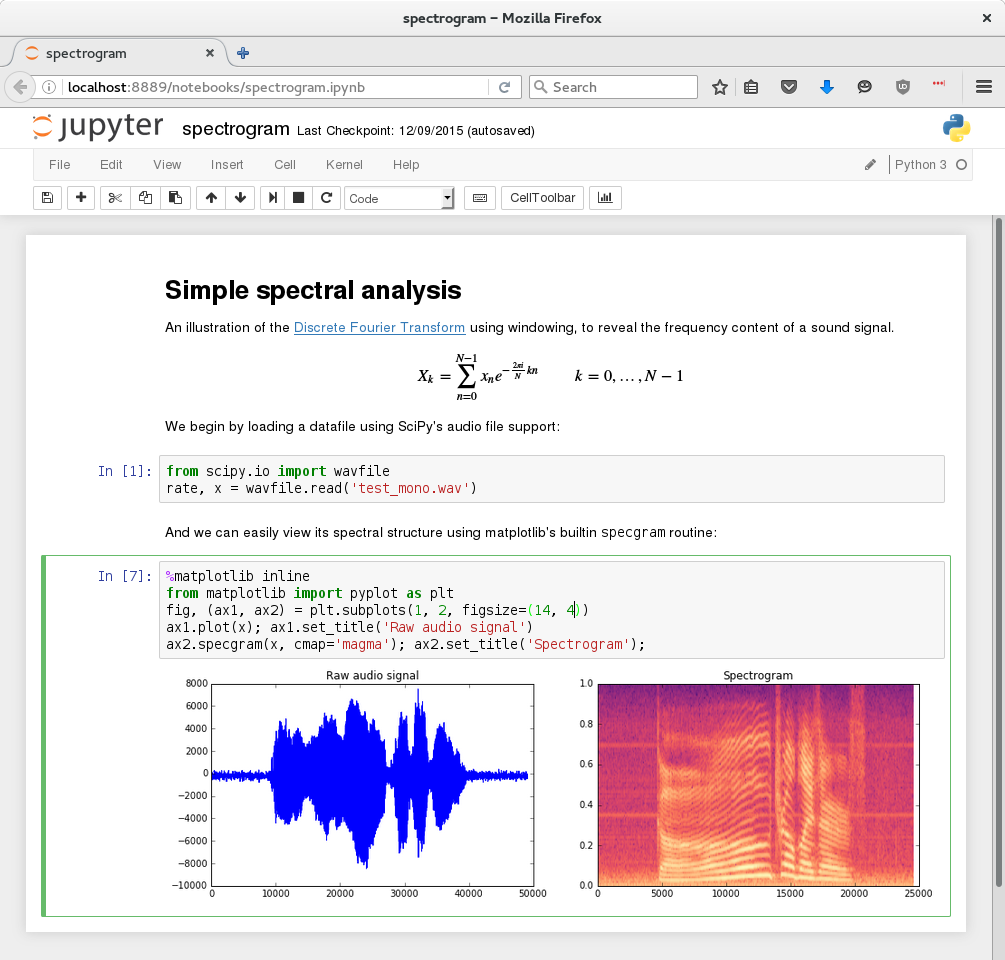
\includegraphics[width=0.9\textwidth]{spectrogram_smaller.png}
  \caption{A notebook document in the Jupyter Notebook interface.}\label{fig:notebook-screenshot}
\end{figure}

\begin{itemize}
  \item The \textbf{Jupyter Notebook} is the flagship application of Project Jupyter.
  It allows the creation of notebook documents, containing a mixture of text and
  interactively executable code, along with rich output from running that code.
  Figure \ref{fig:notebook-screenshot} shows an open notebook including graphs
  from an audio processing example. Notebook documents are readily shareable,
  providing a popular way to describe and illustrate computational methods and
  tools.
  \textbf{JupyterLab} is the new, modular, extensible client application
  for Jupyter notebooks.

  \item \textbf{Jupyter kernels} are the backend software which allow Jupyter to execute
  code in many different programming languages. The \textbf{IPython} kernel is
  the reference kernel, supporting the Python programming language, and is
  developed by the Jupyter core team. Kernels for other languages are maintained
  by third parties.

  \item \textbf{nbconvert} converts notebook files to a variety of other file
  formats, including HTML and PDF, so that the content of a notebook can easily
  be shared with people who don't have Jupyter software. nbconvert also powers
  \textbf{nbviewer}, a web service which provides static HTML views of publicly
  accessible notebooks.

  \item \textbf{JupyterHub} is a multi-user extension of the Jupyter Notebook.
  It runs on one or more notebook servers, for example at a research institution.
  Users can log in to author and run notebooks securely through their web
  browser, without needing to install any special software on their own
  computer.

\end{itemize}

\subsubsection{Jupyter ecosystem}
\label{jupyter-ecosystem}

While Jupyter is a large, distributed, coordinated project,
the wider community of Jupyter users develops a great deal of
software with Jupyter integration,
providing increased or domain-specific functionality,
building on top of Jupyter, or integrating core Jupyter components in some aspect.
We call this the \textbf{Jupyter ecosystem}.
The broader Jupyter ecosystem includes many more projects than we will describe
here, but a selection of projects which may be relevant to
\TheProject includes:

\begin{itemize}

  \item \textbf{Binder} builds on JupyterHub to allow sharing executable
  environments along with data files and a description of the libraries
  required to run the notebooks. When someone accesses a Binder repository,
  the service builds the computational environment on-demand, allowing them to
  execute and modify a copy of the notebooks.
  \textbf{repo2docker} \cite{repo2docker} and \textbf{BinderHub} \cite{binder} are components of the Binder
  software.

  \item \textbf{nbsphinx} \cite{Nbsphinx} integrates notebooks with the \emph{Sphinx}
  documentation system, which is widely used for software documentation,
  especially but not only for software written in Python.
  This allows developers to write notebooks showing how to use a library,
  then seamlessly make those notebooks part of their main documentation.

  \item \textbf{nbval} \cite{nbval} is a plugin for the popular \emph{pytest} testing
  framework to automatically execute notebooks and optionally check that the
  output matches that saved in the file. While this is not a subsitute for a
  test suite, it's valuable for documentation with code examples in notebooks.
  If changes to the underlying tools mean the example no longer
  works, testing with nbval will quickly show this, so that either the software
  or the example can be corrected. This ensures that example code doesn't
  get outdated.

  \item \textbf{nbdime} \cite{nbdime} provides tools for comparing and merging notebooks.
  These integrate with version control systems such as \emph{git}, which
  are designed for plain text files and typically don't handle notebook files
  well.

  \item \textbf{Widgets} allow interactive output in the notebook which can
  communicate with the kernel, updating values in the kernel and updating the
  displayed output as code runs. \textbf{ipywidgets} \cite{ipywidgets} provides the main
  implementation for the IPython kernel, while other packages such as
  \textbf{bqplot} \cite{bqplot}, \textbf{ipyvolume} \cite{ipyvolume} and
  \textbf{K3D} \cite{K3D} extend the framework to provide 2D and 3D visualisations.
  Figure \ref{fig:ipywidgets-example} shows a simple example of interactive
  widgets in use.

  \item The \textbf{Voila} package \cite{Voila} enables the
  sharing of notebook-based interactive dashboards for non-technical users.

  \item The \textbf{Xeus} instrastructure \cite{Corlay2017} supports writing kernels
  in C++. \textbf{xeus-cling} is one such kernel, running user code in C++,
  and built upon CERN's C++ interpreter, "cling" \cite{Vassilev2012},
  which has a lot of adoption in the High-Energy-Physics community.
  xeus-cling is already in use for teaching the C++ programming language.
\end{itemize}

\begin{figure}[ht]\centering
  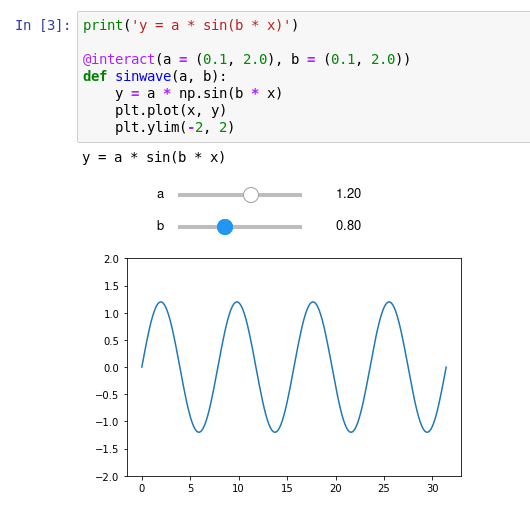
\includegraphics[width=0.6\textwidth]{ipywidgets_example.png}
  \caption{An example of using two simple slider widgets to explore the
  parameter space of a function. The \texttt{@interact} decorator creates
  the widgets and connects them to the function.}
  \label{fig:ipywidgets-example}
\end{figure}

\subsection{This proposal}

In this proposal, core team developers of the project, including a
number of recipients of the ACM award, and key contributors to the
open source scientific computing ecosystem detail improvements to the
capabilities of Project Jupyter.  The goal is to improve the
accessibility of EOSC resources to researchers and the general public,
and improve the accessibility, interactivity, reproducibility and
re-usability of computational research.

\subsubsection{Proposed improvements of core components of Jupyter (WP2)}

We plan to make technical changes to the Jupyter Notebook software to support
real-time collaboration (\taskref{core}{collaboration}),
so that two or more people in different places can work together
on the same notebook. This would significantly enhance the value of
notebooks for collaborative research.
We will also work on making Jupyter software accessible to as broad a
range of users as possible (\taskref{core}{accessibility}).

Further work to bring the code behind JupyterHub and Binder closer together
(\taskref{core}{jh-bh-conv}) will bring a range of benefits, allowing more
flexible sharing of notebooks along with access to remote computing resources
such as EOSC.

Finally, we are explicitly allocating time in \WPref{core} for maintaining
Jupyter software, as well as new development (\taskref{core}{maintenance}).
Maintenance is crucial to creating reliable, sustainable software,
but its cost is often swept under the rug in funding applications
because of the perceived pressure to focus on novelty.

\subsubsection{Proposed improvements of the Jupyter ecosystem (WP3)}

We further propose improvements of the wider Jupyter ecosystem for
better scientific workflows. In particular, we have identified
possible improvements to:

\begin{itemize}
  \item Binder and its crucial software component \emph{repo2docker}
    (\taskref{ecosystem}{r2d-and-binder})

  \item Xeus, to better support the C++ programming language in notebooks
    (\taskref{ecosystem}{xeus-cpp})

  \item Interactive widgets, including tools for 3D visualisation to help
    people make sense of large amounts of data (\taskref{ecosystem}{jupyter-widgets})
\end{itemize}

\WPref{ecosystem} also includes work on tooling and guidelines for using
notebooks in education (\taskref{ecosystem}{teaching-tools}),
and for archiving computational environments to allow reproducible research
with a focus on the long term (\taskref{ecosystem}{reproducibility}).
We may create new open source software projects in these tasks,
but we will carefully review existing existing software, both in the
Jupyter ecosystem and beyond, to avoid unnecessary duplication of effort.

\subsubsection{Beyond the improvement of the Jupyter Project (WP4,
  WP5, WP6)}
Beyond the improvement to the software stack, we plan on
\begin{itemize}
\item Application, demonstration and evaluation of such novel services
  in multiple demonstrators, that cover research fields such as
  health, astrophysics, photon and neutron science, geosciences and
  mathematics, and also interests of participating SMEs (WP4)
\item Operating a \emph{European Binder Service} on the EOSC-hub and
  enabling provision of Jupyter Services through the EOSC-sub (WP5).
\item Producing \emph{training and education material} to disseminate
  the ability to do reproducible computational science using the tools
  we develop, among others. (WP6)
\end{itemize}

\clearpage

%%% Local Variables:
%%% mode: latex
%%% TeX-master: "proposal"
%%% End:
